%% =====================================================================
%% PRE-INFORME PRÁCTICA 3 — Electrónica Análoga I (2026-II)
%% Diodo Zener y amplificadores operacionales
%% Formato IEEE doble columna (IEEEtran). Máx. 7 páginas sin referencias.
%% =====================================================================
\documentclass[conference]{IEEEtran}

\usepackage[utf8]{inputenc}
\usepackage[T1]{fontenc}
\usepackage[spanish]{babel}
\usepackage{amsmath,amssymb}
\usepackage{graphicx}
\usepackage{booktabs}
\usepackage{array}
\usepackage{siunitx}
\usepackage{xcolor}
\usepackage{cite}
\usepackage{placeins}
\usepackage[hyphens]{url}
\urlstyle{same}

\sisetup{output-decimal-marker={.}, group-minimum-digits=5}
% Punto decimal también en modo matemático con babel-spanish
\providecommand{\decimalpoint}{}
\AtBeginDocument{\decimalpoint}
\addto\captionsspanish{\renewcommand{\figurename}{Fig.}\renewcommand{\tablename}{Tabla}}

% Rutas corregidas respetando mayúsculas/minúsculas del árbol de archivos
\graphicspath{{./}{Figuras/}{figuras/}{imagenes/}}

% --- Atajos de unidades (siempre con unidades) ---
\newcommand{\qV}[1]{\SI{#1}{\volt}}
\newcommand{\qmA}[1]{\SI{#1}{\milli\ampere}}
\newcommand{\qohm}[1]{\SI{#1}{\ohm}}
\newcommand{\qkohm}[1]{\SI{#1}{\kilo\ohm}}
\newcommand{\qmW}[1]{\SI{#1}{\milli\watt}}
\newcommand{\qW}[1]{\SI{#1}{\watt}}

% --- Marcador visible para las partes de los compañeros ---
\newcommand{\PEND}[2]{\par\smallskip\noindent\fcolorbox{red}{yellow!25}{\parbox{\dimexpr\columnwidth-2\fboxsep-2\fboxrule}{\footnotesize\textbf{[#1 --- PENDIENTE]} #2}}\par\smallskip}

\begin{document}

\title{Pre-informe Práctica 3: Diodo Zener como Regulador de Tensión y Configuraciones Básicas con Amplificadores Operacionales}

\author{
\IEEEauthorblockN{Juan José Tobar Álvarez}
\IEEEauthorblockA{Universidad Nacional de Colombia\\
jutobara@unal.edu.co}
\and
\IEEEauthorblockN{Nombre Apellido (Persona 2)}
\IEEEauthorblockA{Universidad Nacional de Colombia\\
correo2@unal.edu.co}
\and
\IEEEauthorblockN{Nombre Apellido (Persona 3)}
\IEEEauthorblockA{Universidad Nacional de Colombia\\
correo3@unal.edu.co}
}

\maketitle

%% =====================================================================
\section{Introducción/Justificación}
%% =====================================================================

\subsection{Introducción}
En esta práctica se estudia el diodo Zener como regulador de tensión y las configuraciones básicas de amplificadores operacionales (inversor, no inversor y sumador inversor). El objetivo general es determinar la característica $I$--$V$ del diodo Zener y diseñar tanto reguladores de tensión como etapas de amplificación. Los objetivos específicos son: (i) comprobar el modelo característico del Zener, (ii) diseñar fuentes de tensión constante ante variaciones de la entrada o de la carga y (iii) estudiar el funcionamiento del inversor, el no inversor y el sumador-inversor. Los conceptos y leyes empleados son las leyes de Ohm y de Kirchhoff, la región de ruptura inversa del Zener, el modelo de amplificador operacional ideal (ganancia infinita y cortocircuito virtual) y el concepto de ancho de banda \cite{sedra}. Este pre-informe reúne las consultas, los cálculos de diseño y los esquemáticos de simulación previos a la ejecución del laboratorio.

\subsection{Justificación}
Los reguladores con diodo Zener y los amplificadores operacionales se emplean en sistemas donde la confiabilidad es crítica. En el sector aeroespacial, la NASA documentó un regulador de tensión DC cuya referencia es un diodo Zener \cite{nasa}, y se han evaluado reguladores shunt con Zener a temperaturas criogénicas porque algunas misiones espaciales exponen la electrónica a temperaturas muy inferiores al rango especificado por el fabricante \cite{cryo}. Los amplificadores operacionales son bloques básicos de la electrónica de una nave: miden tensiones del bus de potencia y almacenan en buffer las señales antes de un conversor análogo-digital \cite{tispace}; una nave mediana puede tener más de 500 sensores que requieren amplificadores de instrumentación tolerantes a la radiación, construidos con arreglos de amplificadores operacionales \cite{renesas}. En la industria médica, el electrocardiograma (ECG) necesita acondicionar biopotenciales muy pequeños mediante amplificadores operacionales y amplificadores diferenciales \cite{penn}.

Por tanto, la práctica es importante porque entrena el dimensionamiento de resistencias y potencias para fuentes de tensión estables, así como el diseño de etapas de ganancia que no saturen, competencias necesarias en instrumentación, potencia y acondicionamiento de señales.

\subsection{Marco teórico y consultas previas}
\textbf{1) Hojas de datos.} En la Tabla~\ref{tab:zener_ds} se resumen los parámetros de los Zener usados, tomados de la hoja de datos de la serie 1N4728A--1N4764A \cite{fairchild}. Se adopta $I_{ZM}$ como corriente máxima del regulador; para el 1N4738A, $I_{ZM}=\qmA{110}$ es más restrictiva que $P_D/V_Z=\qmA{122}$.

\begin{table}[htbp]
\caption{Parámetros de los diodos Zener \cite{fairchild}}
\label{tab:zener_ds}
\centering
\footnotesize
\begin{tabular}{lcc}
\toprule
Parámetro & 1N4738A & 1N4733A \\
\midrule
$V_Z$ a $I_{ZT}$ (tolerancia $\pm5\%$) & \qV{8.2} & \qV{5.1} \\
$I_{ZT}$ (corriente de prueba) & \qmA{31} & \qmA{49} \\
$Z_{ZT}$ (impedancia dinámica) & \qohm{4.5} & \qohm{7} \\
$I_{ZK}$ (corriente de codo) & \qmA{0.5} & \qmA{1} \\
$I_{ZM}$ (corriente máxima) & \qmA{110} & \qmA{178} \\
$P_D$ máxima (a $T_L\le \SI{50}{\celsius}$) & \qW{1} & \qW{1} \\
\bottomrule
\end{tabular}
\end{table}

\textbf{2) Polarización y aplicaciones.} En polarización inversa, superada la tensión de ruptura el Zener conduce y mantiene $V_Z$ casi constante aunque cambie la corriente; en polarización directa se comporta como un diodo común (caída cercana a \qV{0.7}). Esto permite usarlo como regulador, referencia de tensión y protección contra sobretensión \cite{sedra}.

\textbf{3) Conexión como regulador.} El Zener se conecta inversamente en paralelo con la carga y se alimenta a través de una resistencia serie $R_1$. Por la ley de corrientes de Kirchhoff, $I_{R1}=I_Z+I_L$, y el diseño exige $I_Z\ge I_{ZK}$ (para mantenerse en ruptura) y $P_Z=V_ZI_Z\le P_{Z,\max}$ \cite{sedra}.

\textbf{4) Tensiones de los amplificadores operacionales.} La Tabla~\ref{tab:opamp_ds} resume los límites de alimentación según las hojas de datos del LM324 \cite{lm324,lm324n} y del LF353 \cite{lf353}. La salida no puede superar los rieles: en el LM324 la excursión positiva se limita a $V^{+}-\qV{1.5}$ \cite{lm324n}, por lo que la alimentación debe superar la amplitud de salida requerida sin exceder el máximo del fabricante.

\textbf{5) Funcionamiento y cortocircuito virtual.} Con ganancia de lazo abierto muy alta y realimentación negativa, $v_+\approx v_-$ (cortocircuito virtual) y las corrientes de entrada son despreciables \cite{sedra}. Con ello las ganancias ideales son:
\begin{equation}
G_{NI}=1+\frac{R_2}{R_1},\quad G_{INV}=-\frac{R_2}{R_1},\quad v_o=-R_f\sum_k\frac{v_k}{R_k}.
\label{eq:ganancias}
\end{equation}
La ecuación~\eqref{eq:ganancias} da, en orden, la ganancia del no inversor, del inversor y la salida del sumador inversor.

\textbf{6) Ancho de banda.} El producto ganancia--ancho de banda ($GBW$) es aproximadamente constante, de modo que la frecuencia de corte a $-3\,\mathrm{dB}$ del lazo cerrado es
\begin{equation}
f_{-3\,\mathrm{dB}}\approx\frac{GBW}{1+R_2/R_1}.
\label{eq:bw}
\end{equation}
La ecuación~\eqref{eq:bw} indica que a mayor ganancia, menor ancho de banda \cite{sedra}. La Tabla~\ref{tab:opamp_ds} incluye los valores esperados para los circuitos diseñados, que servirán de referencia para la simulación (estimación a partir del $GBW$ típico).

\begin{table}[htbp]
\caption{Límites y ancho de banda esperado de los amplificadores}
\label{tab:opamp_ds}
\centering
\footnotesize
\begin{tabular}{lcc}
\toprule
Parámetro & LM324 \cite{lm324,lm324n} & LF353 \cite{lf353} \\
\midrule
Alimentación máxima & \qV{32} (\SI{\pm16}{\volt}) & \SI{\pm18}{\volt} \\
$GBW$ típico & \SI{1.2}{\mega\hertz} & \SI{4}{\mega\hertz} \\
Slew rate típico & \SI{0.5}{\volt\per\micro\second} & \SI{13}{\volt\per\micro\second} \\
$f_{-3\,\mathrm{dB}}$ inversor ($|G|=2$) & \SI{400}{\kilo\hertz} & \SI{1.33}{\mega\hertz} \\
$f_{-3\,\mathrm{dB}}$ no inversor ($G=4$) & \SI{300}{\kilo\hertz} & \SI{1}{\mega\hertz} \\
\bottomrule
\end{tabular}
\end{table}

\begin{figure*}[!t]
\centering
\begin{minipage}{0.24\textwidth}
  \centering
  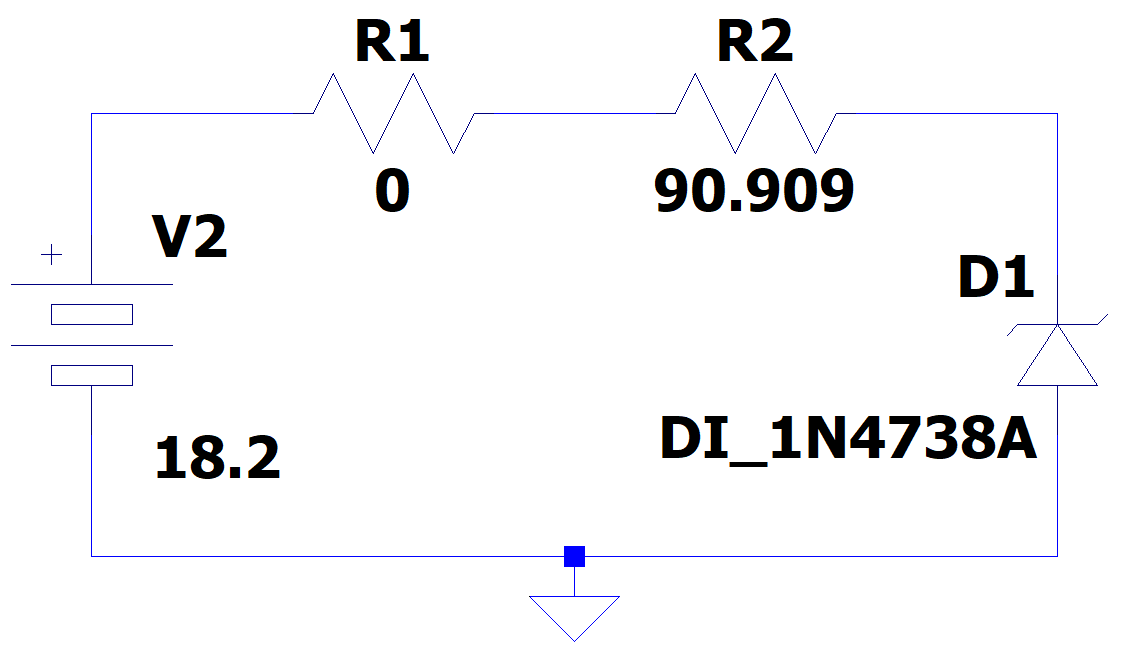
\includegraphics[width=\textwidth]{fig1_zener_nc_R1_0.png}
  \centerline{\footnotesize (a) No com., $R_1=0$}
\end{minipage}\hfill
\begin{minipage}{0.24\textwidth}
  \centering
  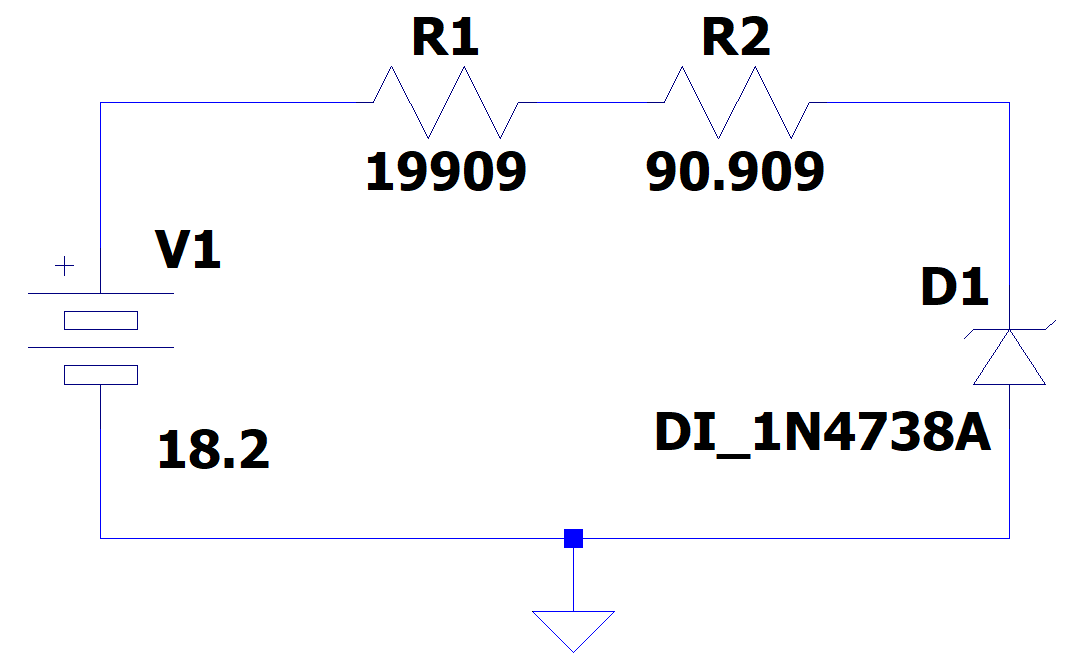
\includegraphics[width=\textwidth]{fig1_zener_nc_R1max.png}
  \centerline{\footnotesize (b) No com., $R_{1\max}$}
\end{minipage}\hfill
\begin{minipage}{0.24\textwidth}
  \centering
  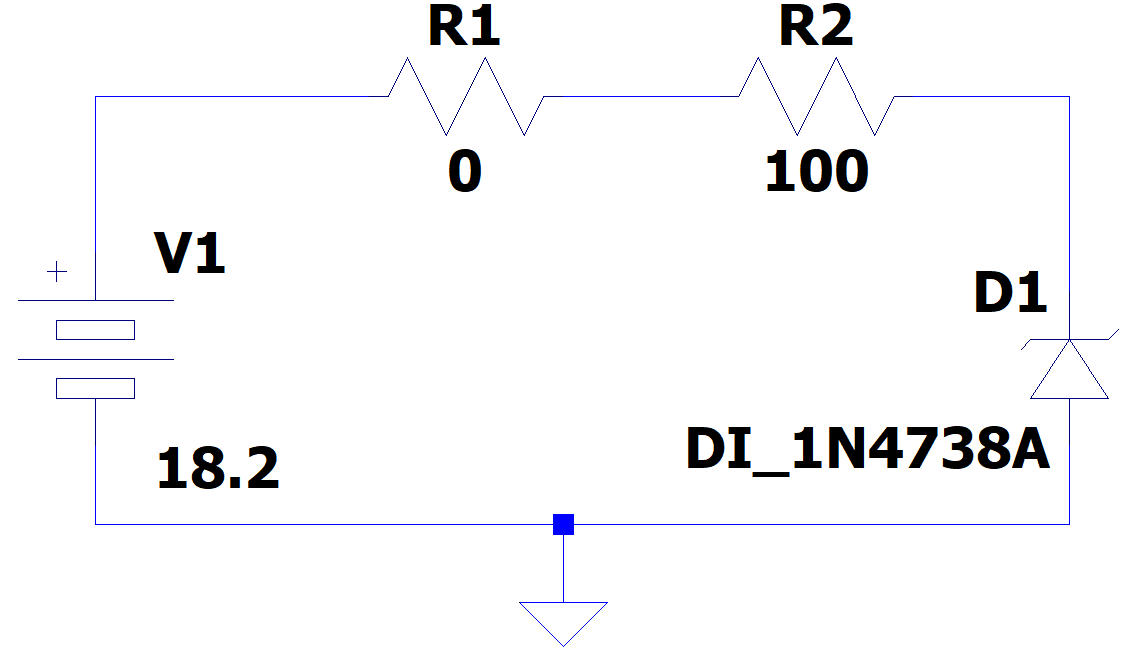
\includegraphics[width=\textwidth]{fig1_zener_com_R1_0.png}
  \centerline{\footnotesize (c) Com., $R_1=0$}
\end{minipage}\hfill
\begin{minipage}{0.24\textwidth}
  \centering
  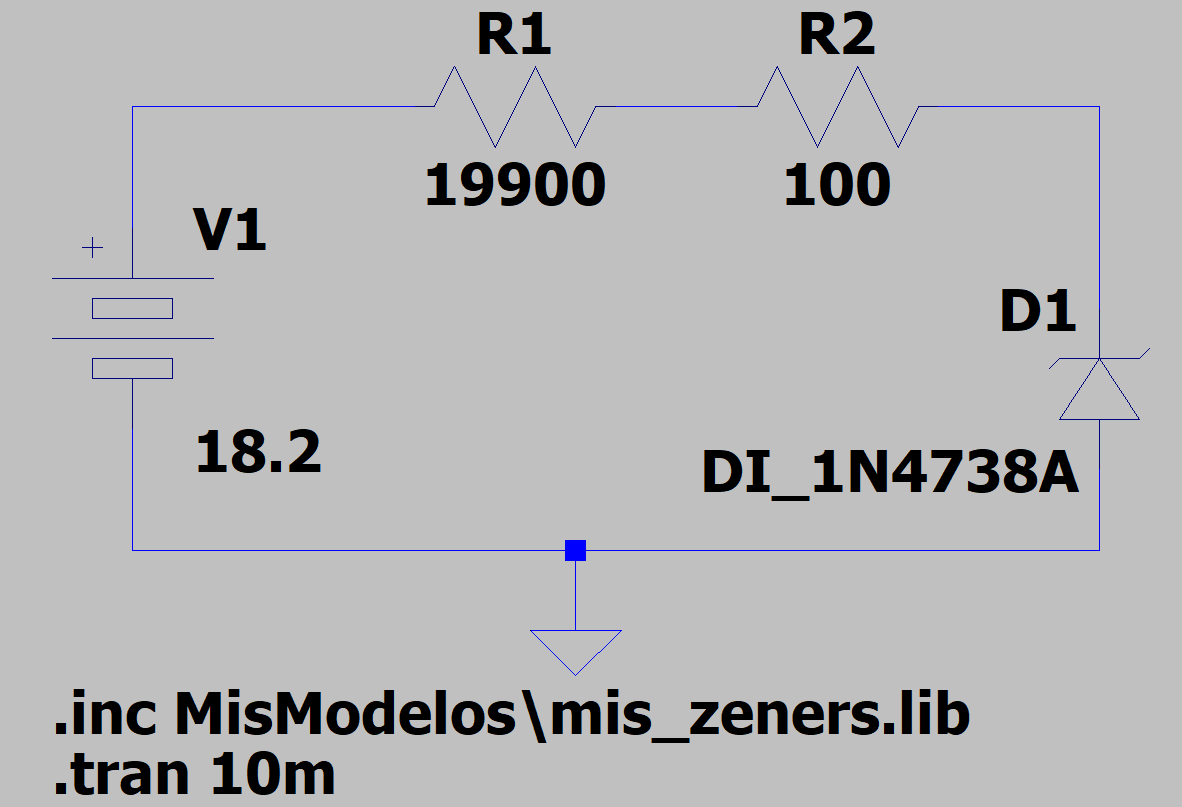
\includegraphics[width=\textwidth]{fig1_zener_com_R1max.png}
  \centerline{\footnotesize (d) Com., $R_{1\max}$}
\end{minipage}
\caption{Esquemáticos del circuito de caracterización con 1N4738A ($V_1=\qV{18.2}$): (a) y (b) valores no comerciales; (c) y (d) valores comerciales.}
\label{fig:zener1}
\end{figure*}

%% =====================================================================
\section{Cálculos}
%% =====================================================================

\subsection{Regulador de caracterización con 1N4738A}
En el circuito de caracterización de la guía (esquemáticos en la Fig.~\ref{fig:zener1}) se tiene $V_1=V_Z+\qV{10}=\qV{18.2}$, de modo que \qV{10} caen en $R_1+R_2$. Con $R_1=\qohm{0}$ toda la corriente fija $R_2$, y se exige $I_Z<I_{ZM}$:
\begin{equation}
R_2=\frac{V_1-V_Z}{I_{ZM}}=\frac{\qV{10}}{\qmA{110}}=\qohm{90.909}.
\label{eq:R2}
\end{equation}
La ecuación~\eqref{eq:R2} es el valor mínimo de $R_2$ que no sobrepasa la corriente máxima del diodo. Para $R_1=R_{1\max}$ se exige $I_Z\approx I_{ZK}=\qmA{0.5}$:
\begin{equation}
R_{1\max}=\frac{V_1-V_Z}{I_{ZK}}-R_2=\frac{\qV{10}}{\qmA{0.5}}-\qohm{90.909}=\qohm{19909}.
\label{eq:R1max}
\end{equation}
La ecuación~\eqref{eq:R1max} indica la resistencia serie a partir de la cual el Zener sale del codo de la curva. Las potencias en cada elemento se obtienen de
\begin{equation}
P_R=I^{2}R,\qquad P_Z=V_ZI_Z,\qquad P_{V_1}=V_1I.
\label{eq:pot}
\end{equation}

\textbf{Valores comerciales.} Como $R_2=\qohm{90.909}$ no es comercial (el valor más cercano de la serie E24 es \qohm{91}, que deja un margen casi nulo), se adopta $R_2=\qohm{100}$ (serie E12), con lo que $I_Z=\qV{10}/\qohm{100}=\qmA{100}$, es decir, $-9.09\%$ respecto a \qmA{110}, quedando por debajo de $I_{ZM}$. Para $R_{1\max}$ se usa $\qkohm{18}+\qkohm{1.8}+\qohm{100}=\qkohm{19.9}$ en serie; junto con $R_2$ suma \qkohm{20}, igual que en el caso no comercial ($\qohm{19909}+\qohm{90.909}$), por lo que $I_Z=\qmA{0.5}$ no cambia. La Tabla~\ref{tab:zener1} muestra los resultados.

\begin{table}[htbp]
\caption{Corriente y potencias del circuito de caracterización ($V_1=\qV{18.2}$, valores ideales con $V_Z=\qV{8.2}$)}
\label{tab:zener1}
\centering
\scriptsize
\setlength{\tabcolsep}{3pt}
\begin{tabular}{llrrrrrrr}
\toprule
Caso & & $R_1$ & $R_2$ & $I_Z$ & $P_{R1}$ & $P_{R2}$ & $P_Z$ & $P_{V1}$ \\
 & & ($\Omega$) & ($\Omega$) & (mA) & (mW) & (mW) & (mW) & (mW) \\
\midrule
No com. & $R_1=0$ & 0 & 90.909 & 110 & 0 & 1100 & 902 & 2002 \\
No com. & $R_{1\max}$ & 19909 & 90.909 & 0.5 & 4.977 & 0.023 & 4.1 & 9.1 \\
Com. & $R_1=0$ & 0 & 100 & 100 & 0 & 1000 & 820 & 1820 \\
Com. & $R_{1\max}$ & 19900 & 100 & 0.5 & 4.975 & 0.025 & 4.1 & 9.1 \\
\bottomrule
\end{tabular}
\end{table}

Con $R_1=0$, $R_2$ disipa \qW{1} y el Zener \qW{0.82}, cercano a su límite de \qW{1} (la hoja de datos indica una reducción de \SI{6.67}{\milli\watt\per\celsius} por encima de \SI{50}{\celsius} \cite{fairchild}); por ello $R_2$ debe ser de \qW{2} (carga del 50\%) y el Zener requiere buena ventilación. En el caso de $R_{1\max}$ cada resistencia disipa menos de \qmW{5}, por lo que basta con \qW{0.25}. La fuente debe suministrar al menos \qW{1.82} (\qV{18.2}, \qmA{100}).

\textbf{Efecto de la impedancia dinámica.} Si $V_Z$ crece con la corriente, $\Delta V_Z\approx Z_{ZT}(I_Z-I_{ZT})=\qohm{4.5}\cdot(\qmA{110}-\qmA{31})\approx\qV{0.36}$, de modo que en simulación se espera $I_Z\approx\qmA{106}$ en el caso $R_1=0$, algo menor que el valor ideal.

\subsection{Fuente regulada con 1N4733A}
Con $V_Z=\qV{5.1}$, $I_{ZM}=\qmA{178}$, $I_{ZK}=\qmA{1}$ y $P_{Z,\max}=V_ZI_{ZM}=\qW{0.908}$, la carga $R_2=\qohm{150}$ demanda
\begin{equation}
I_L=\frac{V_Z}{R_L}=\frac{\qV{5.1}}{\qohm{150}}=\qmA{34},\qquad P_L=\qmW{173.4}.
\label{eq:IL}
\end{equation}
La ecuación~\eqref{eq:IL} es la corriente (casi constante) que el Zener debe dejar pasar a la carga. Aplicando la ley de corrientes, $I_{R1}=I_Z+I_L$, el intervalo de $R_1$ para $V_1=\qV{12}$ es
\begin{align}
R_{1\min}&=\frac{V_1-V_Z}{I_{ZM}+I_L}=\frac{\qV{6.9}}{\qmA{212}}=\qohm{32.547},\label{eq:R1min}\\
R_{1\max}&=\frac{V_1-V_Z}{I_{ZK}+I_L}=\frac{\qV{6.9}}{\qmA{35}}=\qohm{197.143}.\label{eq:R1max2}
\end{align}
Las ecuaciones~\eqref{eq:R1min} y \eqref{eq:R1max2} fijan los límites por potencia máxima del Zener y por pérdida de regulación, respectivamente. Con $V_1=\qV{5}<V_Z$ el Zener no alcanza la ruptura: con $R_1=0$ la carga recibe \qV{5} (\qmA{33.3}) y no hay regulación posible, sea cual sea $R_1$.

\textbf{Elección.} En los extremos $P_{R1}=\qW{1.463}$ (con $R_{1\min}$) y \qW{0.242} (con $R_{1\max}$). Se elige $R_1=\qohm{100}$ (serie E12), dentro del intervalo y cerca de su punto medio ($\approx\qohm{115}$), con lo que $I_{R1}=\qmA{69}$, $I_Z=\qmA{35}$ y $P_{R1}=\qW{0.476}$ a \qV{12}. Con carga desconectada, $I_Z=\qmA{69}$ y $P_Z=\qmW{352}<\qW{0.908}$. La tensión mínima de regulación es $V_{1,\min}=V_Z+R_1(I_{ZK}+I_L)=\qV{8.6}$ y la máxima antes de superar $I_{ZM}$ es $V_Z+R_1(I_{ZM}+I_L)=\qV{26.3}$. Los puntos de operación de laboratorio ($V_1=5$, 9 y \qV{12}) se resumen en la Tabla~\ref{tab:zener2}.

\begin{figure}[!t]
\centering
\begin{minipage}{0.48\columnwidth}
  \centering
  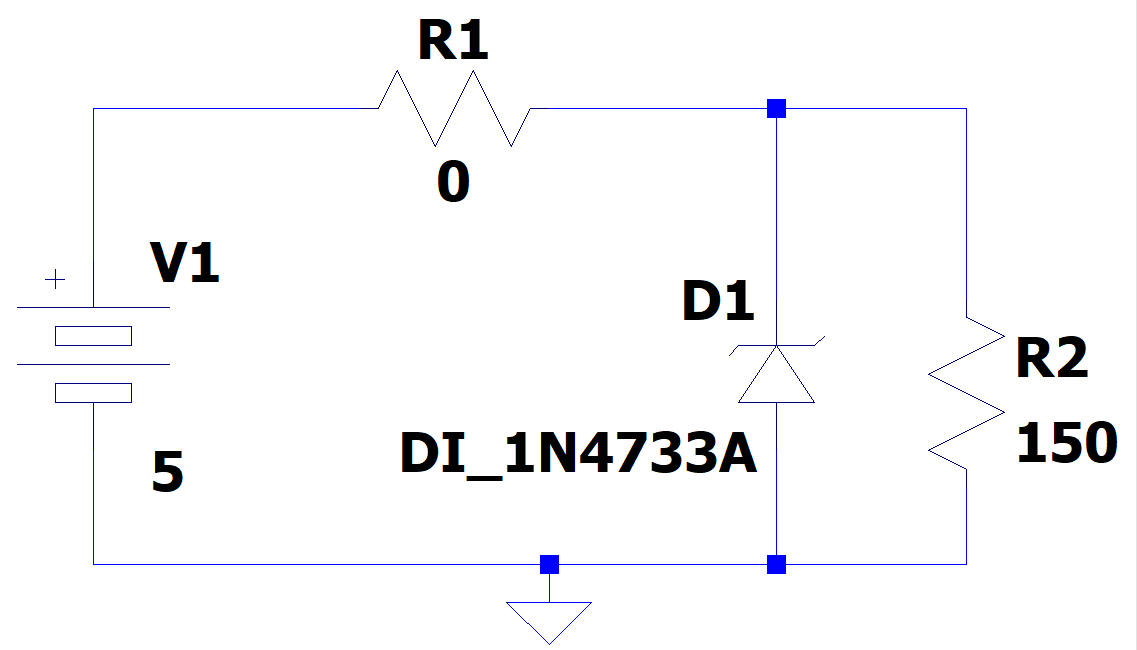
\includegraphics[width=\textwidth]{fig2_regulador_5V.png}
  \centerline{\footnotesize (a) $V_1=\qV{5}$, $R_1=0$}
\end{minipage}\hfill
\begin{minipage}{0.48\columnwidth}
  \centering
  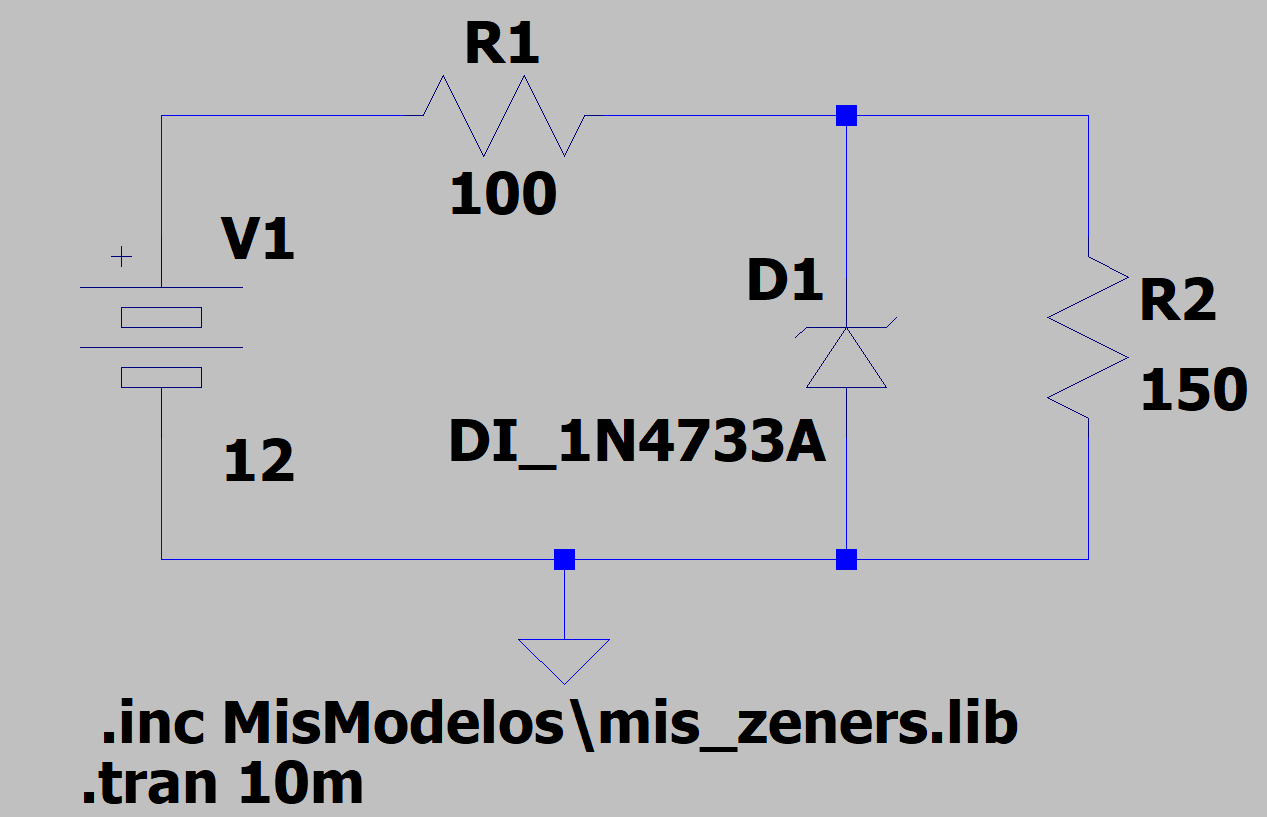
\includegraphics[width=\textwidth]{fig2_regulador_12V.png}
  \centerline{\footnotesize (b) $V_1=\qV{12}$, $R_1=\qohm{100}$}
\end{minipage}
\caption{Esquemáticos del regulador con 1N4733A y carga $R_2=\qohm{150}$.}
\label{fig:zener2}
\end{figure}

\begin{table}[htbp]
\caption{Puntos de operación del regulador ($V_Z=\qV{5.1}$, $R_L=\qohm{150}$)}
\label{tab:zener2}
\centering
\scriptsize
\setlength{\tabcolsep}{2.5pt}
\begin{tabular}{rrrrrrrrr}
\toprule
$V_1$ & $R_1$ & $V_o$ & $I_{R1}$ & $I_Z$ & $P_{R1}$ & $P_Z$ & $P_L$ & $P_{V1}$ \\
(V) & ($\Omega$) & (V) & (mA) & (mA) & (mW) & (mW) & (mW) & (mW) \\
\midrule
5 & 0 & 5.00 & 33.3 & 0 & 0 & 0 & 166.7 & 166.7 \\
5 & 100 & 3.00 & 20.0 & 0 & 40.0 & 0 & 60.0 & 100.0 \\
9 & 100 & 5.10 & 39.0 & 5.0 & 152.1 & 25.5 & 173.4 & 351.0 \\
12 & 100 & 5.10 & 69.0 & 35.0 & 476.1 & 178.5 & 173.4 & 828.0 \\
\bottomrule
\end{tabular}
\end{table}

Para $V_1=\qV{12}$ la eficiencia es $P_L/P_{V1}=\qmW{173.4}/\qmW{828}=20.9\%$. Como $P_{R1}=\qW{0.476}$ es el $47.6\%$ de \qW{1}, se usa $R_1$ de \qW{1}; $R_2=\qohm{150}$ disipa \qmW{173.4}, por lo que se usa de \qW{0.5}; el Zener, con \qmW{178.5}, trabaja muy por debajo de \qW{1}.

\subsection{Amplificador no inversor}
Para $v_{o,p}=\qV{12}$ con $v_{i,p}=\qV{3}$ se requiere $G_{NI}=12/3=4=1+R_2/R_1$ según \eqref{eq:ganancias}, es decir $R_2=3R_1$: $R_1=\qkohm{10}$ y $R_2=\qkohm{30}$. La resistencia de la entrada no inversora se toma $R_3=R_1\parallel R_2=\qkohm{7.5}$. La alimentación debe cumplir
\begin{equation}
v_{o,p}+\qV{1.5}\le V_{CC}\le\qV{16}\;\Rightarrow\;V_{CC}=\pm\qV{14},
\label{eq:vcc}
\end{equation}
donde \qV{1.5} es el margen respecto al riel del LM324 \cite{lm324n} y \qV{16} es el máximo por polaridad del LM324 (el del LF353 es \SI{\pm18}{\volt}). La ecuación~\eqref{eq:vcc} deja $\qV{14}-\qV{1.5}=\qV{12.5}\ge\qV{12}$ de excursión.

\subsection{Amplificador inversor}
Para $2\,V_{pp}$ de salida con $1\,V_{pp}$ de entrada, $|G_{INV}|=R_2/R_1=2$ según \eqref{eq:ganancias}: $R_1=\qkohm{10}$ y $R_2=\qkohm{20}$, con salida desfasada \SI{180}{\degree} y resistencia de entrada $R_{in}=R_1=\qkohm{10}$. Se mantiene $V_{CC}=\pm\qV{14}$ (dentro del máximo de ambos integrados).

\subsection{Sumador inversor}
Con $R_1=R_2=R_f=R=\qkohm{10}$, la ecuación~\eqref{eq:ganancias} da $v_o=-(v_{in1}+v_{in2})$. Si ambas señales cuadradas están en fase, $v_{o,p}=\qV{1}+\qV{1.5}=\qV{2.5}$, como se pide ($v_{in1}$: $2\,V_{pp}$, $v_{in2}$: $3\,V_{pp}$, \SI{10}{\kilo\hertz}). Para restar una señal basta invertir su polaridad en la entrada. Con $V_{CC}=\pm\qV{5}$, $\qV{5}-\qV{1.5}=\qV{3.5}\ge\qV{2.5}$ (LM324). El cambio de $-\qV{2.5}$ a $+\qV{2.5}$ ($\Delta V=\qV{5}$) con $SR=\SI{0.5}{\volt\per\micro\second}$ \cite{lm324} tardaría $\approx\SI{10}{\micro\second}$ (10\% del periodo de \SI{100}{\micro\second}), efecto que debe observarse en simulación; con el LF353 sería $\approx\SI{0.4}{\micro\second}$ \cite{lf353}.

\begin{figure*}[!t]
\centering
\begin{minipage}{0.31\textwidth}
  \centering
  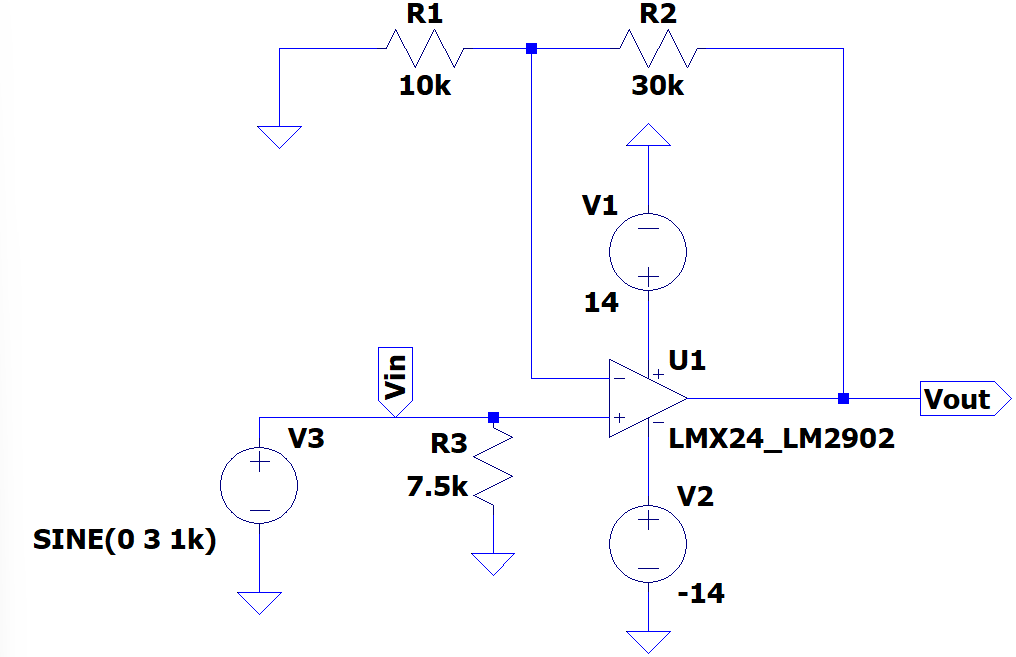
\includegraphics[width=0.95\textwidth]{fig3_noinversor_lm324.png}
  \centerline{\footnotesize (a) No inversor, LM324}
\end{minipage}\hfill
\begin{minipage}{0.31\textwidth}
  \centering
  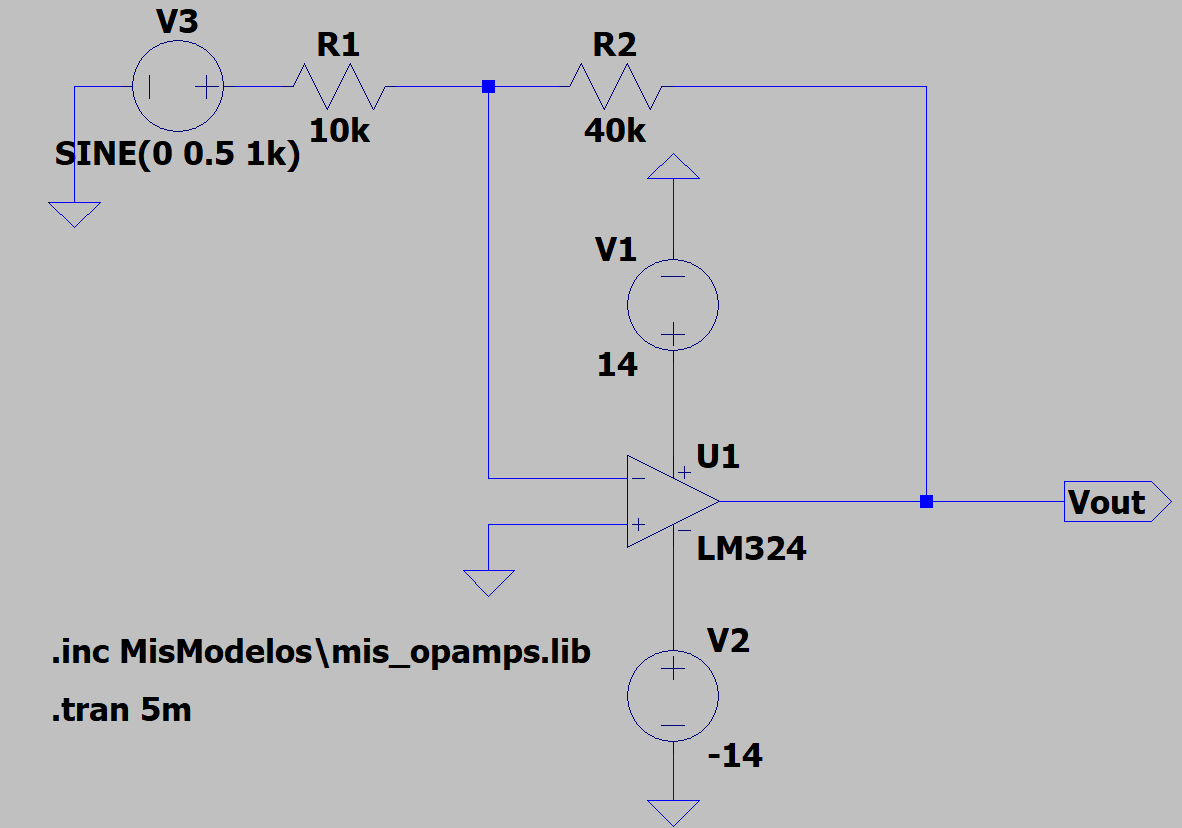
\includegraphics[width=0.95\textwidth]{fig4_inversor_lm324.png}
  \centerline{\footnotesize (b) Inversor, LM324}
\end{minipage}\hfill
\begin{minipage}{0.31\textwidth}
  \centering
  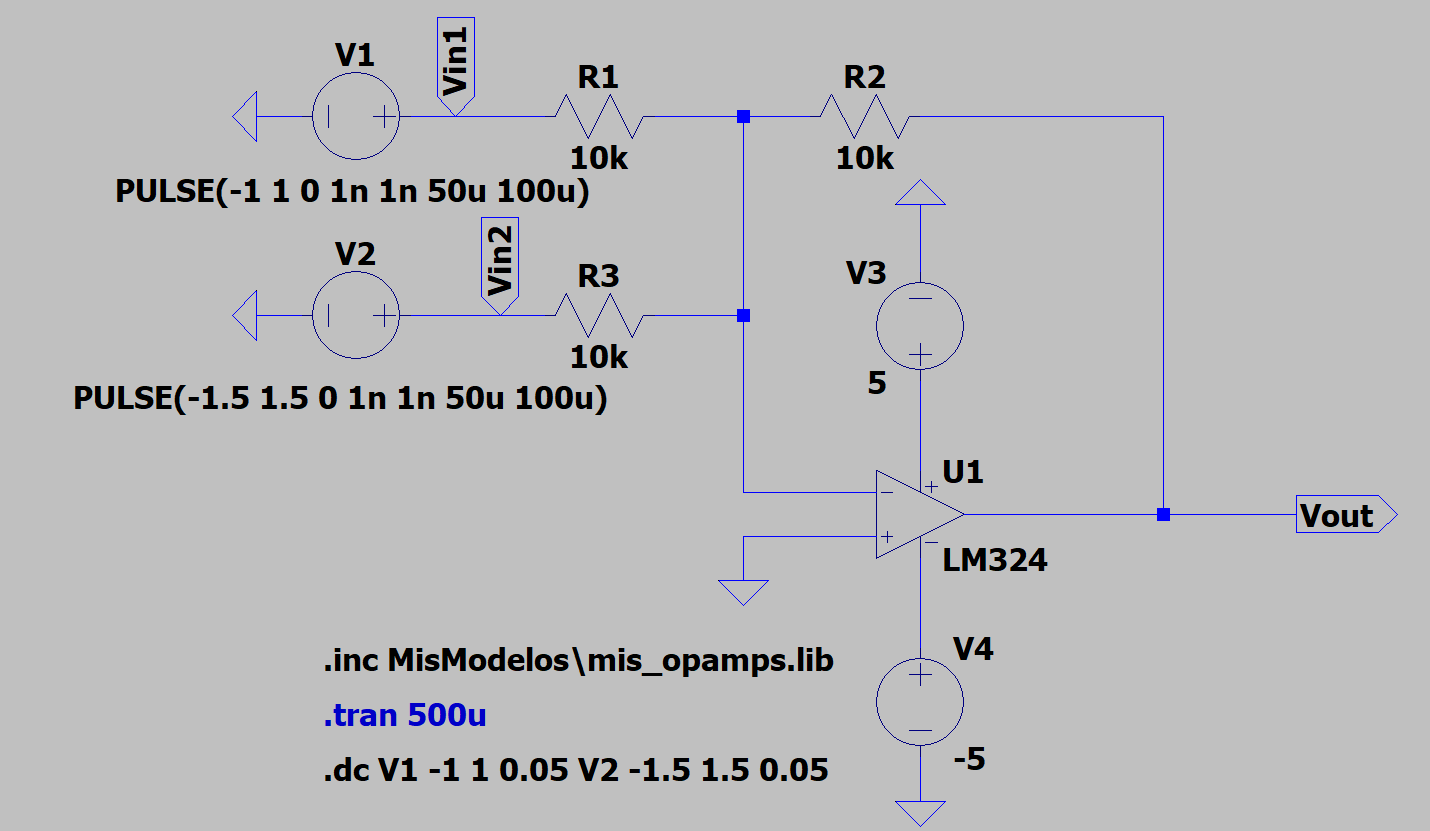
\includegraphics[width=0.95\textwidth]{fig5_sumador_lm324.png}
  \centerline{\footnotesize (c) Sumador, LM324}
\end{minipage}\\[1ex]
\begin{minipage}{0.31\textwidth}
  \centering
  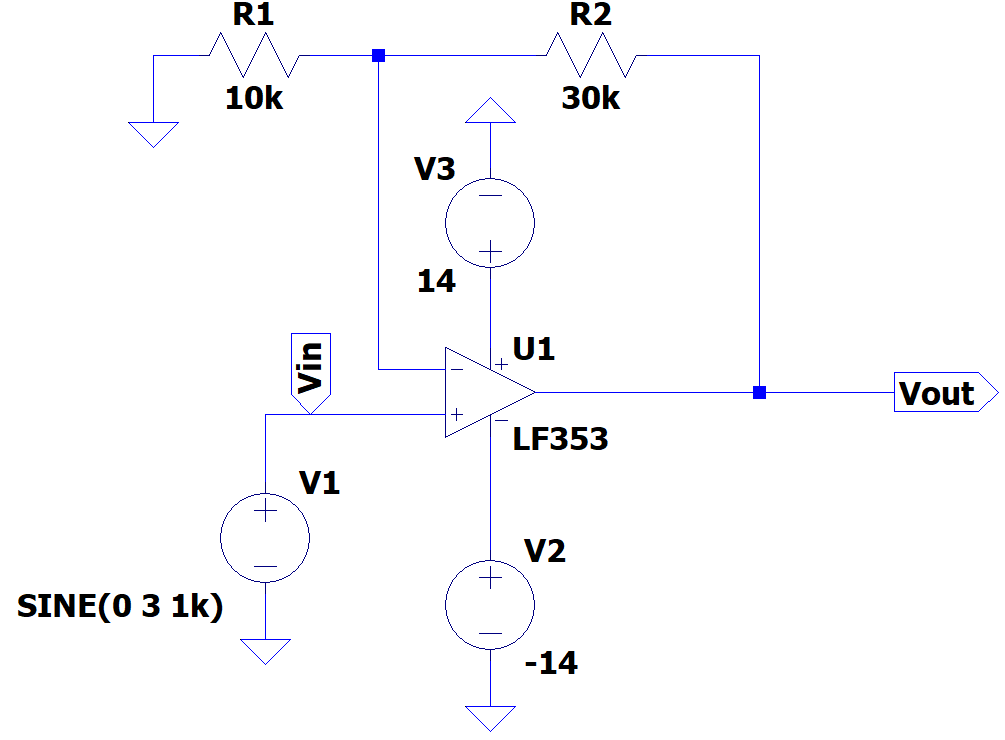
\includegraphics[width=0.95\textwidth]{fig3_noinversor_lf353.png}
  \centerline{\footnotesize (d) No inversor, LF353}
\end{minipage}\hfill
\begin{minipage}{0.31\textwidth}
  \centering
  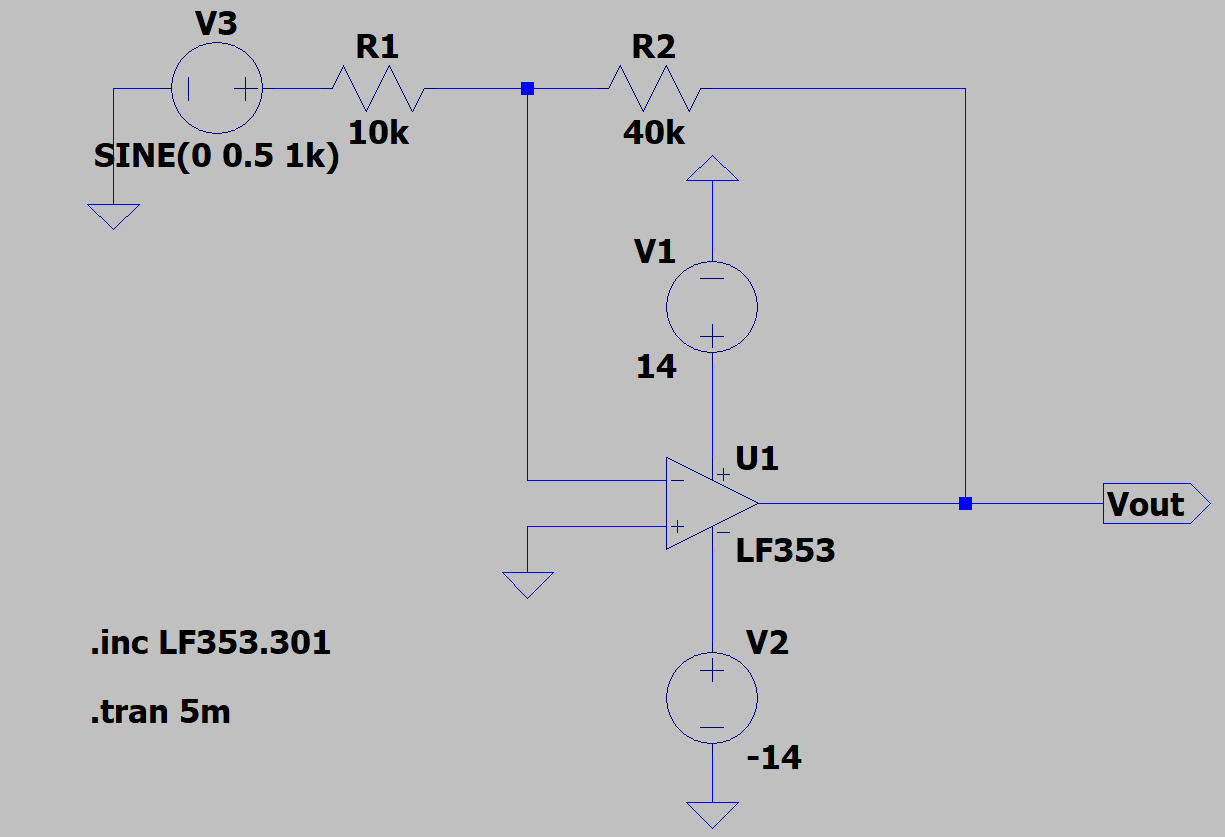
\includegraphics[width=0.95\textwidth]{fig4_inversor_lf353.png}
  \centerline{\footnotesize (e) Inversor, LF353}
\end{minipage}\hfill
\begin{minipage}{0.31\textwidth}
  \centering
  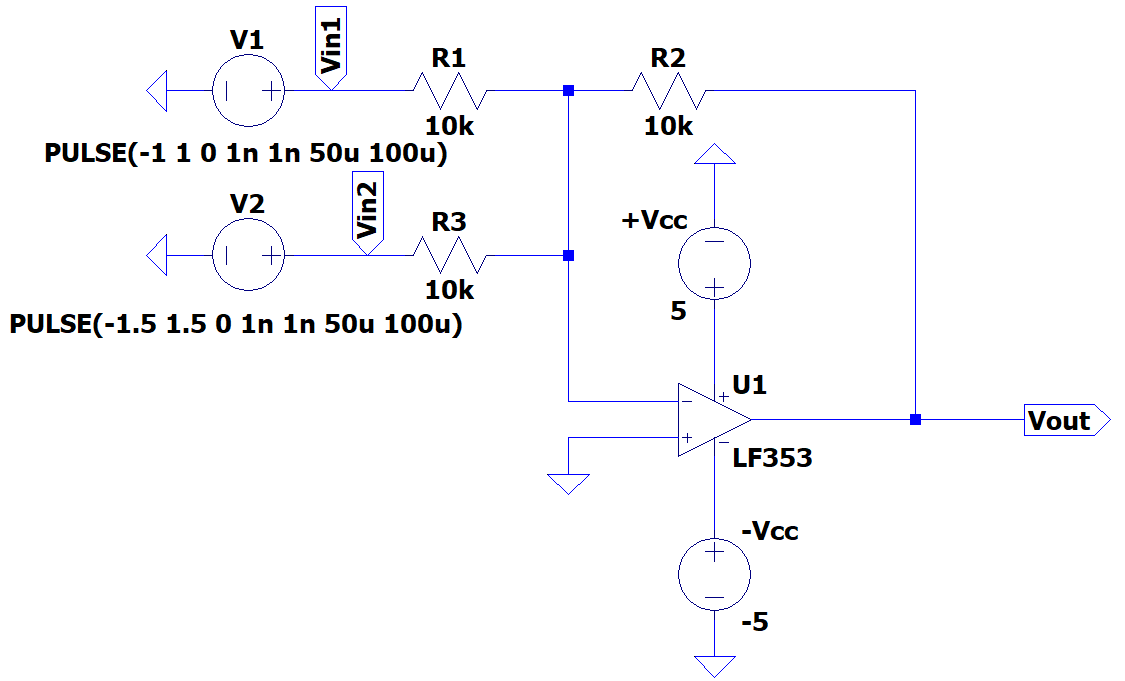
\includegraphics[width=0.95\textwidth]{fig5_sumador_lf353.png}
  \centerline{\footnotesize (f) Sumador, LF353}
\end{minipage}
\caption{Esquemáticos de los circuitos con amplificador operacional: (a)--(c) LM324 y (d)--(f) LF353.}
\label{fig:opamps}
\end{figure*}

La Tabla~\ref{tab:opamps_diseno} resume los diseños con las potencias en los resistores (valores rms para señales sinusoidales; para las cuadradas la potencia es constante).

\begin{table*}[!t]
\caption{Resumen de diseño de los circuitos con amplificador operacional}
\label{tab:opamps_diseno}
\centering
\footnotesize
\begin{tabular}{lccccl}
\toprule
Circuito & Resistencias & $G$ teórica & $V_{CC}$ & $v_{o,p}$ & Potencia en cada resistor \\
\midrule
No inversor & $R_1=\qkohm{10}$, $R_2=\qkohm{30}$, $R_3=\qkohm{7.5}$ & $+4$ & $\pm\qV{14}$ & \qV{12} & $\qmW{0.45}$, $\qmW{1.35}$, $\qmW{0.60}$ \\
Inversor & $R_1=\qkohm{10}$, $R_2=\qkohm{20}$ & $-2$ & $\pm\qV{14}$ & \qV{1} & $\qmW{0.0125}$, $\qmW{0.025}$ \\
Sumador inversor & $R_1=R_2=R_f=\qkohm{10}$ & $-1$ (por entrada) & $\pm\qV{5}$ & \qV{2.5} & $\qmW{0.100}$, $\qmW{0.225}$, $\qmW{0.625}$ ($R_f$) \\
\bottomrule
\end{tabular}
\end{table*}

En todos los casos la potencia es menor que \qmW{1.4}, por lo que se usan resistencias de \qW{0.25}.

%% =====================================================================
\section{Simulación}
%% =====================================================================
Los circuitos se simulan en LTspice con los modelos de la librería indicada en cada esquemático. En la Fig.~\ref{fig:zener1} se muestran los casos del circuito de caracterización, en la Fig.~\ref{fig:zener2} el regulador y en la Fig.~\ref{fig:opamps} los circuitos con amplificador operacional (con LM324 y LF353).

\subsection{Diodos Zener}
\PEND{Persona 2}{Figs. con (1) $I_Z$ extremos del circuito de caracterización (comparar con Tabla~\ref{tab:zener1}); (2) $I_Z$ vs. $R_1$ de \qohm{0} a un máximo; (3) $I_d$ vs. $V_d$ con la tangente en $I_{ZT}$ y $V_Z$; (4) curva de regulación de línea; (5) curva de regulación de carga ($R_2$ de \qohm{100} a \qkohm{1}) y \% de tolerancia.}

\subsection{Amplificadores operacionales}

\FloatBarrier
\subsubsection{Amplificador inversor}
Se comparan las señales de entrada y salida del amplificador inversor para
los modelos LM348 y LF353.
\begin{figure}[!htbp]
\centering
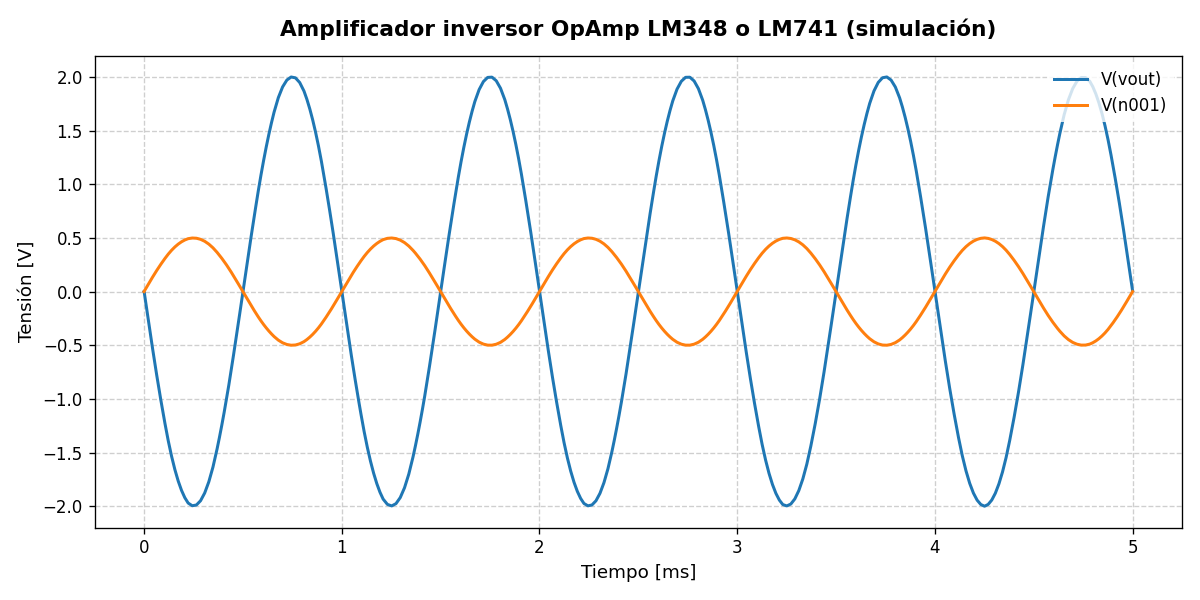
\includegraphics[width=0.55\columnwidth]{simulacion inversor lm348.png}
\caption{Simulación del amplificador inversor con el modelo LM348.}
\label{fig:sim_inversor_lm348}
\end{figure}

\begin{figure}[!htbp]
\centering
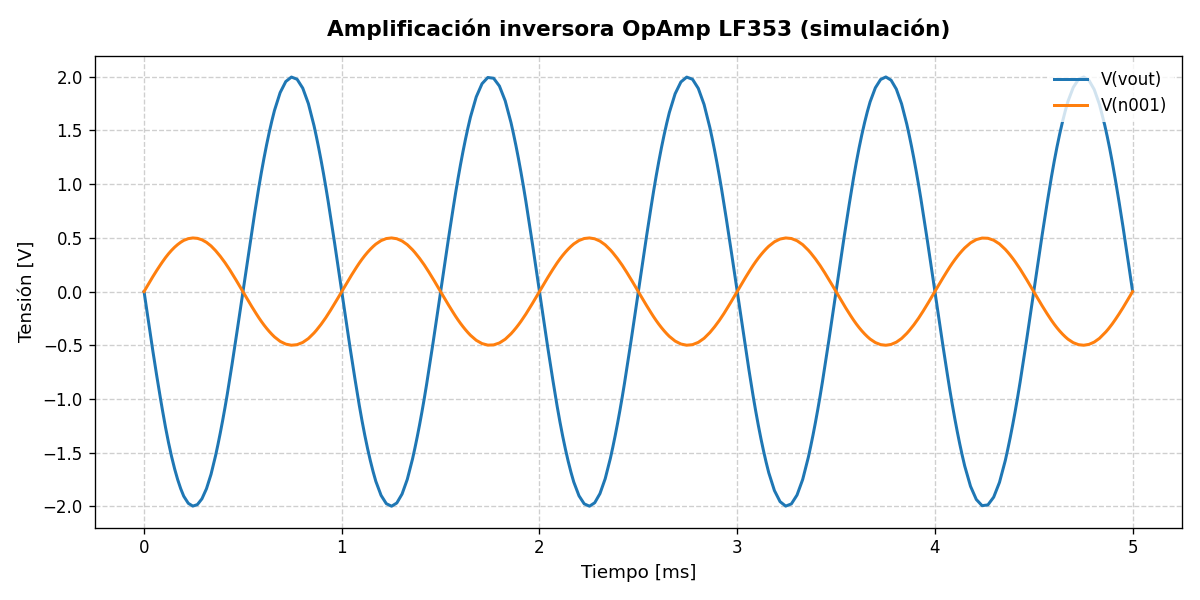
\includegraphics[width=0.55\columnwidth]{simulacion inversor lf353.png}
\caption{Simulación del amplificador inversor con el modelo LF353.}
\label{fig:sim_inversor_lf353}
\end{figure}

\subsubsection{Amplificador no inversor}
Se muestran las señales del amplificador no inversor para los modelos LM348
y LF353 con la alimentación nominal del diseño.
\begin{figure}[!htbp]
\centering
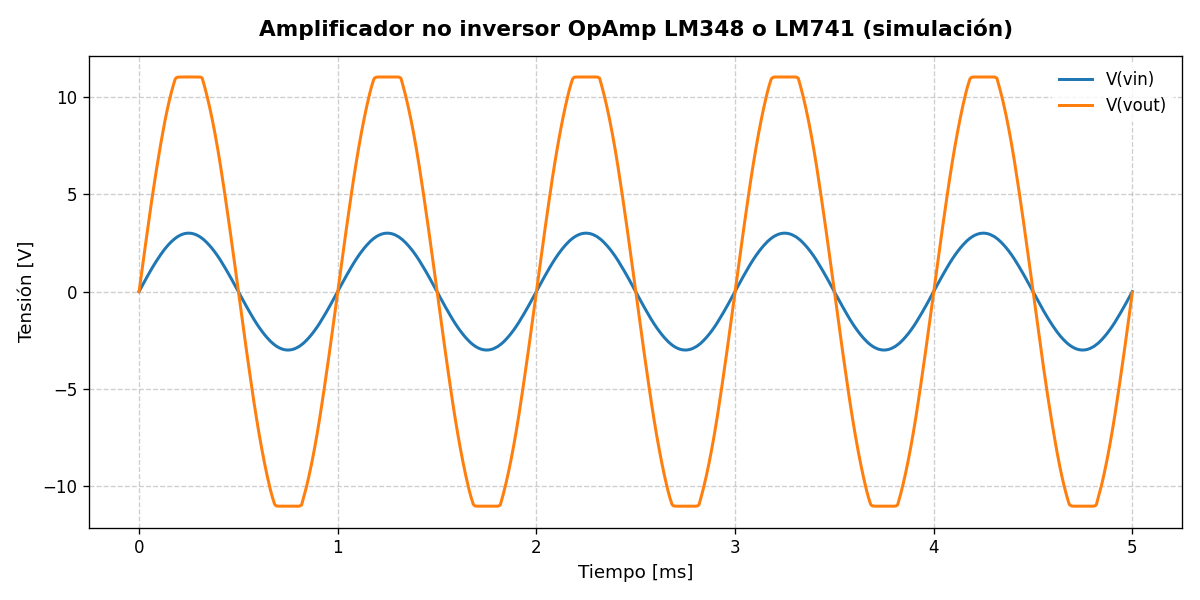
\includegraphics[width=0.55\columnwidth]{simulacion no inversor lm348.png}
\caption{Simulación del amplificador no inversor con el modelo LM348.}
\label{fig:sim_no_inversor_lm348}
\end{figure}

\begin{figure}[!htbp]
\centering
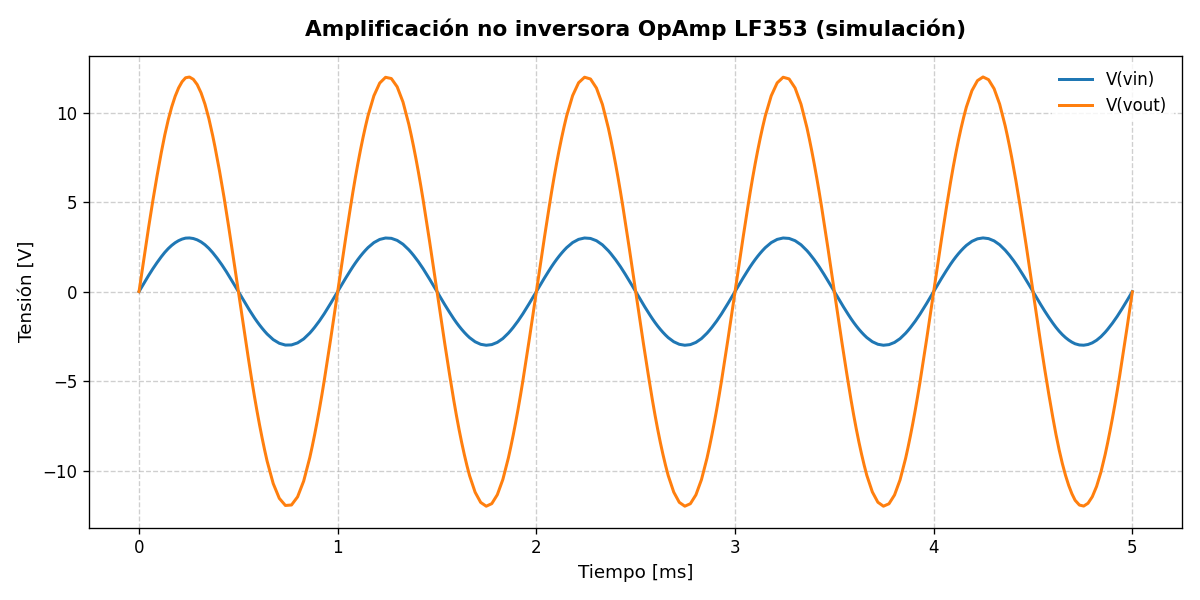
\includegraphics[width=0.55\columnwidth]{simulacion no inversor lf353.png}
\caption{Simulación del amplificador no inversor con el modelo LF353.}
\label{fig:sim_no_inversor_lf353}
\end{figure}

\subsubsection{Amplificador no inversor con variantes en la alimentación}
Se evalúa el efecto de usar alimentación simple y alimentación dual de
\qV{9} en los modelos LM348 y LF353. Se resalta que al disminuirse la tensión de 
polarización frente al $V_p$ de la onda esperada. La onda de salida se ve recortada
a una tensión inferior a la tensión de polarización.

\begin{figure}[!htbp]
\centering
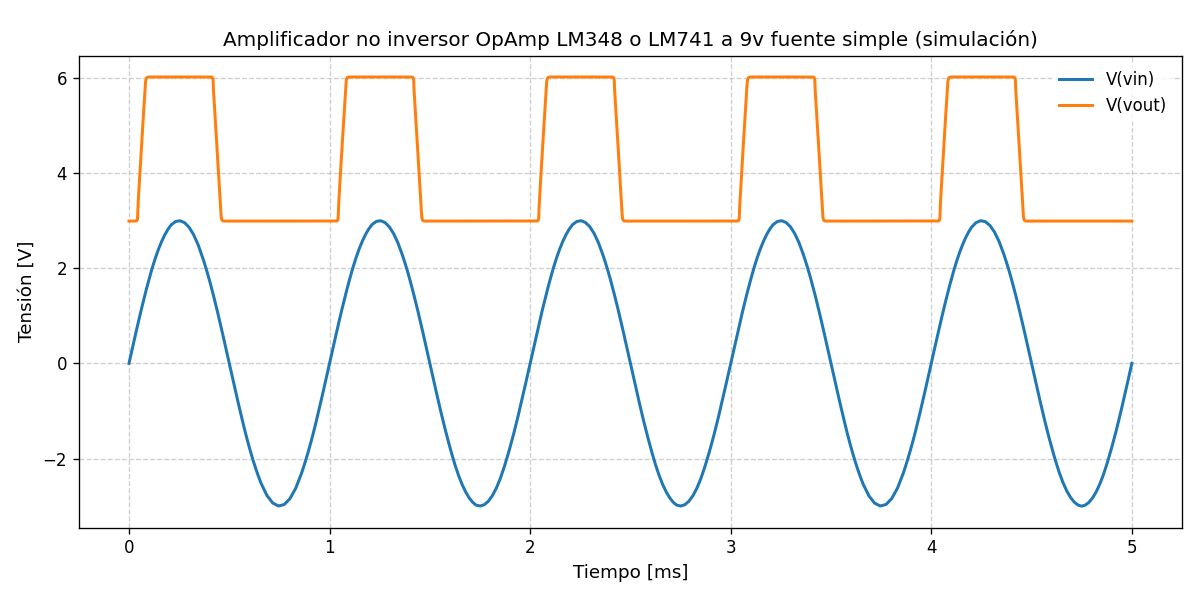
\includegraphics[width=0.55\columnwidth]{simulacion lm348 9v simple.png}
\caption{Amplificador no inversor LM348 con alimentación simple de \qV{9}.}
\label{fig:sim_no_inversor_lm348_9v_simple}
\end{figure}

\begin{figure}[!htbp]
\centering
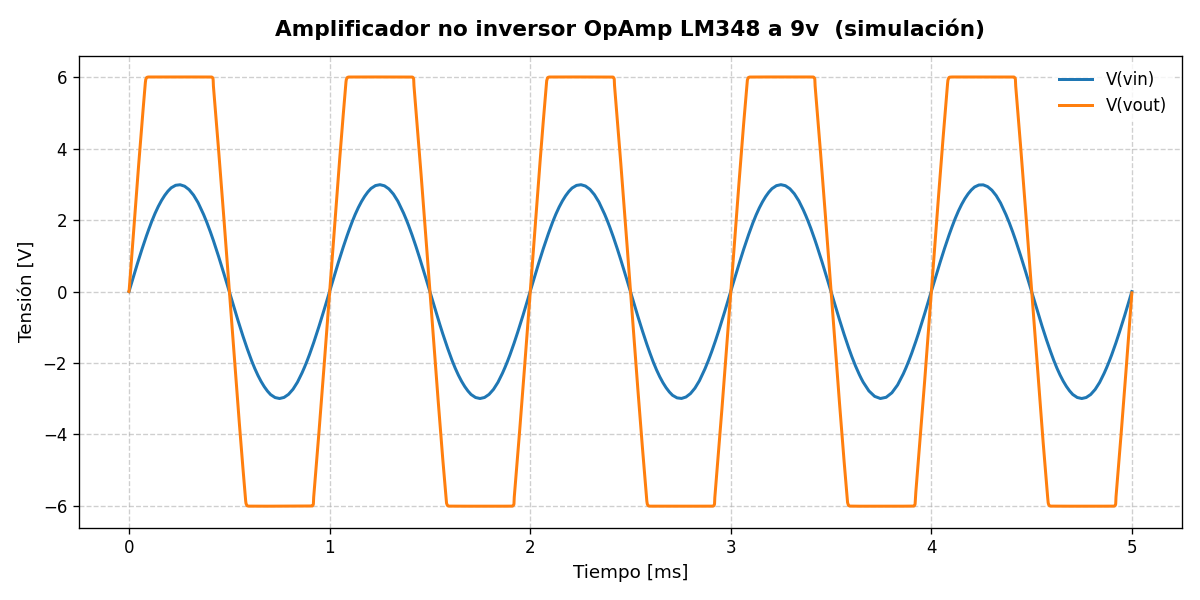
\includegraphics[width=0.55\columnwidth]{simulacion LM348 9v dual.png}
\caption{Amplificador no inversor LM348 con alimentación dual de $\pm\qV{9}$.}
\label{fig:sim_no_inversor_lm348_9v_dual}
\end{figure}

\begin{figure}[!htbp]
\centering
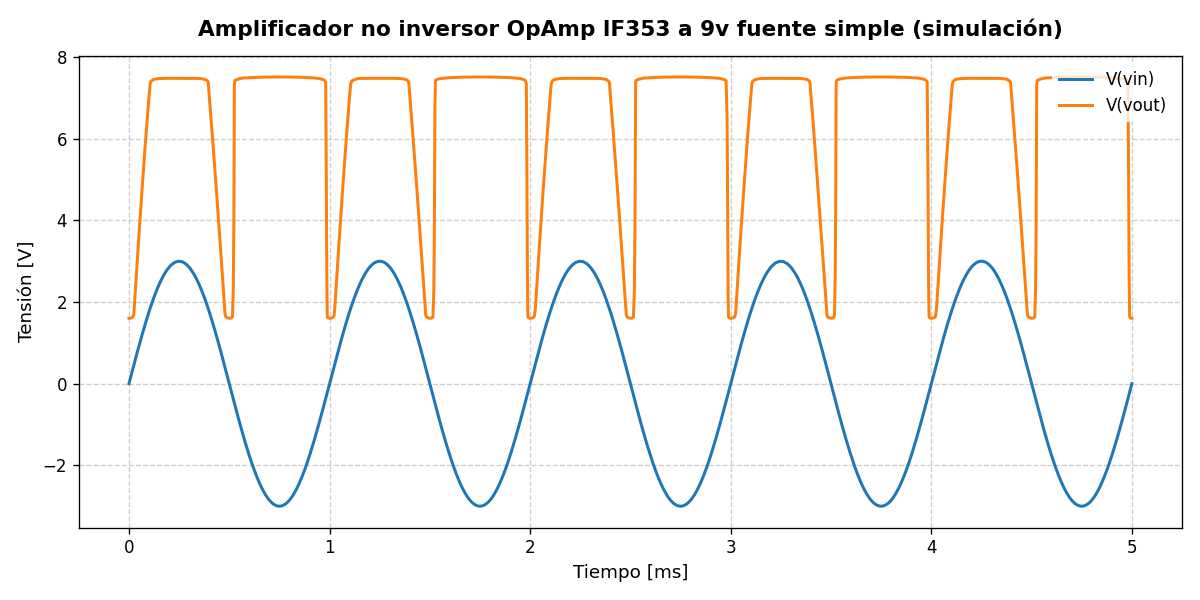
\includegraphics[width=0.55\columnwidth]{simulacion LF353 9v simple .png}
\caption{Amplificador no inversor LF353 con alimentación simple de \qV{9}.}
\label{fig:sim_no_inversor_lf353_9v_simple}
\end{figure}

\begin{figure}[!htbp]
\centering
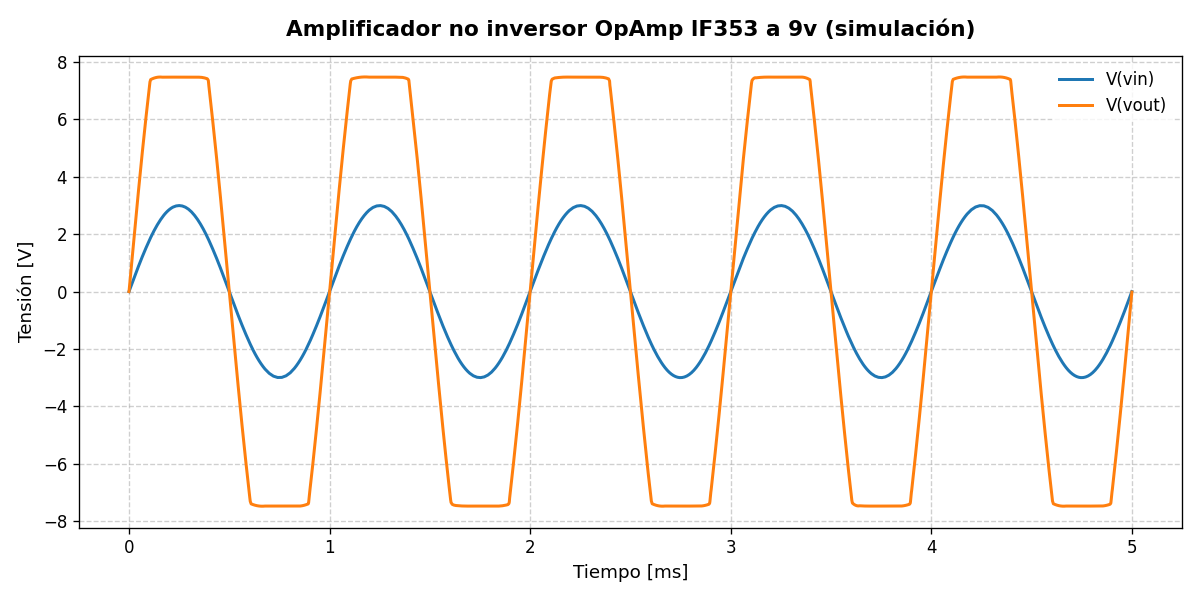
\includegraphics[width=0.55\columnwidth]{simulacion LF353 9v dual.png}
\caption{Amplificador no inversor LF353 con alimentación dual de $\pm\qV{9}$.}
\label{fig:sim_no_inversor_lf353_9v_dual}
\end{figure}

\subsubsection{Amplificador sumador inversor}
Se presentan las formas de onda del sumador inversor implementado con los
modelos LM348 y LF353. A través de esta simulación se nota que el LM348 de
arquitectura basada en BJT, tiene una respuesta mucho más lenta que el LF353 de arquitectura JFET. 
Por lo que el LM348 presenta una onda cuadrada distorsionada. Mientras que el LF353 presenta
una onda cuadrada pura a su salida.
\begin{figure}[!htbp]
\centering
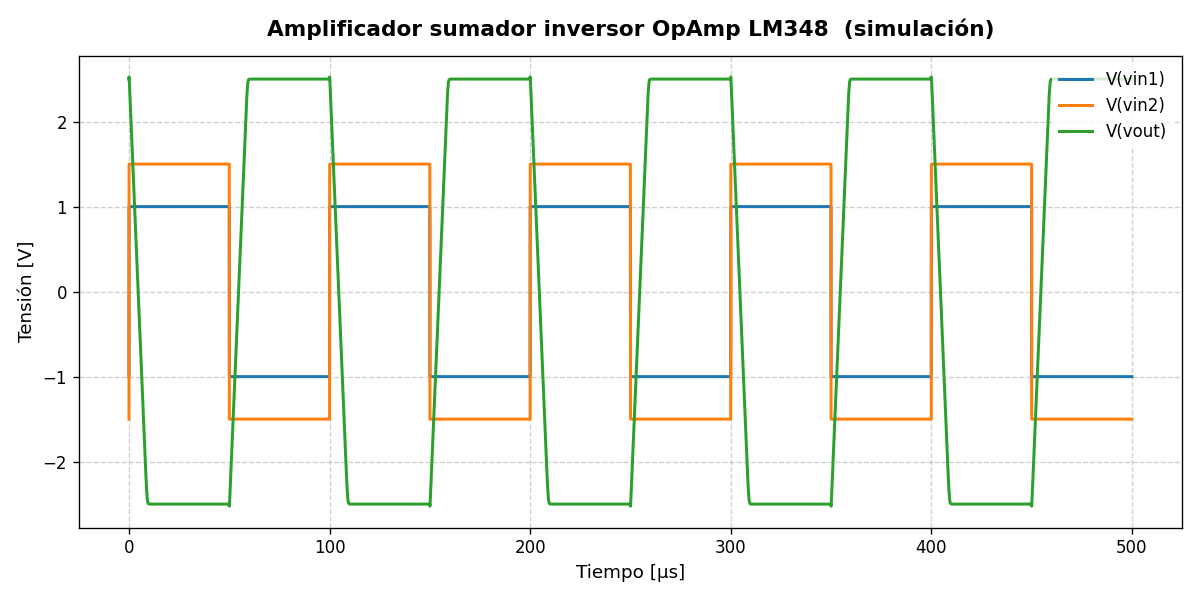
\includegraphics[width=0.55\columnwidth]{simulacion sumador inversor lm348.png}
\caption{Simulación del amplificador sumador inversor con el modelo LM348.}
\label{fig:sim_sumador_lm348}
\end{figure}

\begin{figure}[!htbp]
\centering
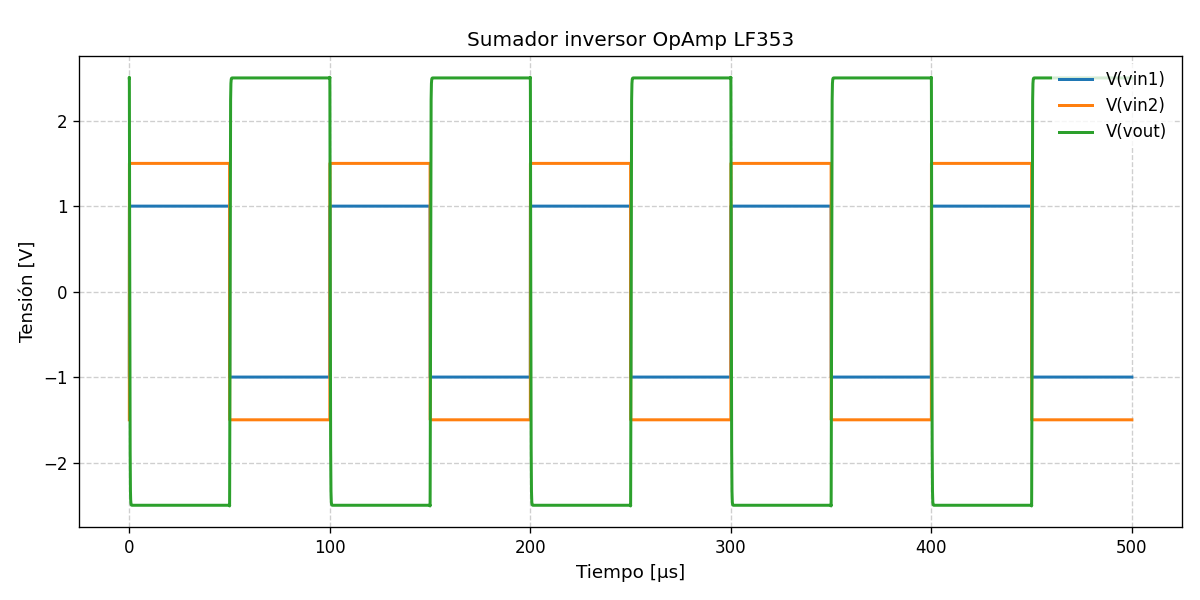
\includegraphics[width=0.55\columnwidth]{simulacion sumador inversor lf353.png}
\caption{Simulación del amplificador sumador inversor con el modelo LF353.}
\label{fig:sim_sumador_lf353}
\end{figure}

\subsubsection{Pruebas de ancho de banda}
Finalmente, se compara la respuesta en frecuencia de los modelos LM348 y
mantiene su ganancia a una frecuencia notablemente más alta que el LM348.
Lo que demuestra a su vez que este tiene más ancho de banda(Según los Datasheet, 3 MHz frente a 1MHz para el LM348)
\begin{figure}[!htbp]
\centering
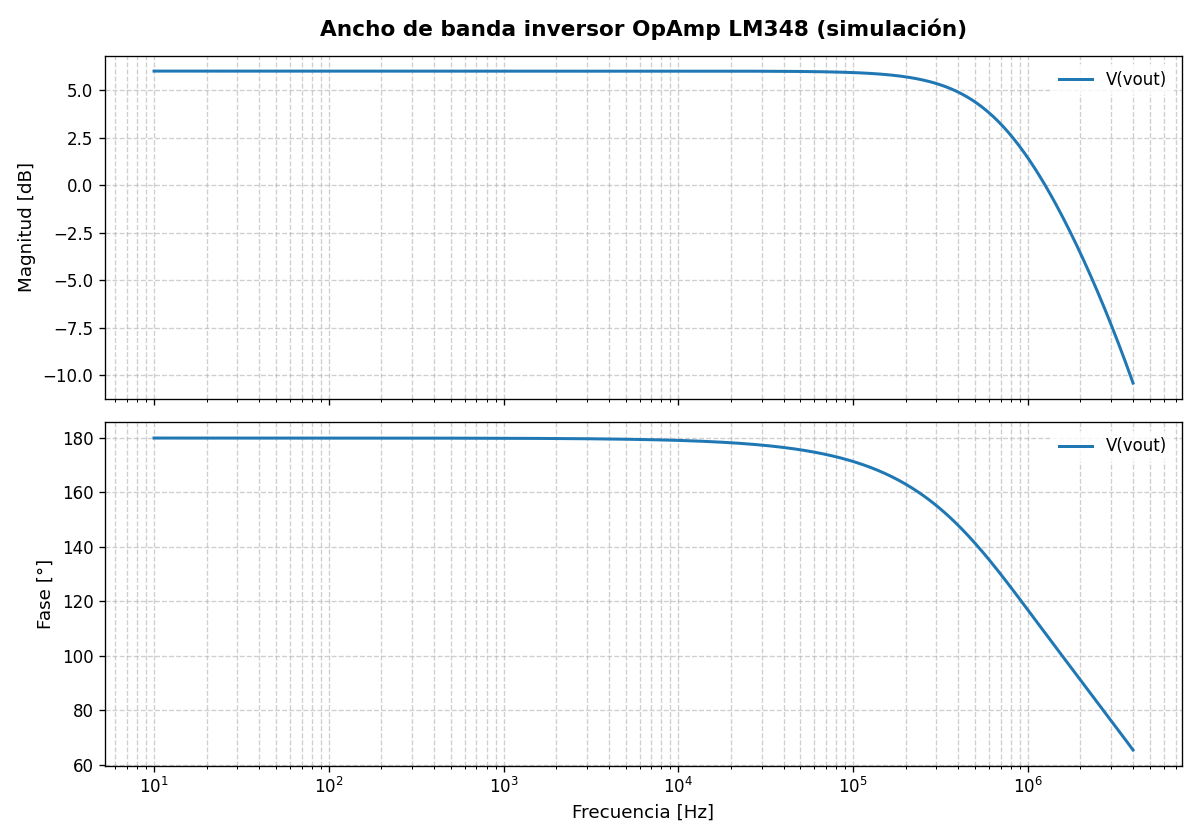
\includegraphics[width=0.55\columnwidth]{simulación BW LM348.png}
\caption{Prueba de ancho de banda con el modelo LM348.}
\label{fig:sim_bw_lm348}
\end{figure}

\begin{figure}[!htbp]
\centering
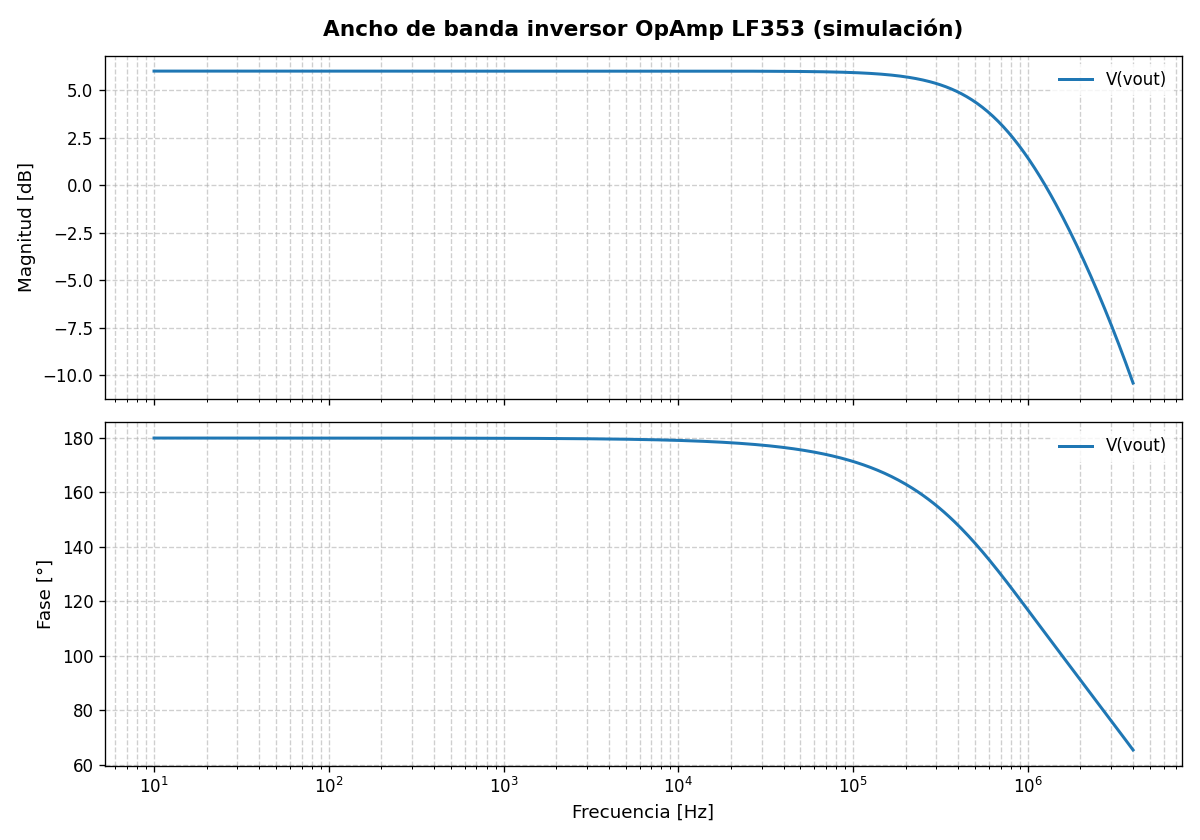
\includegraphics[width=0.55\columnwidth]{simulación BW LF3535.png}
\caption{Prueba de ancho de banda con el modelo LF353.}
\label{fig:sim_bw_lf353}
\end{figure}

\FloatBarrier
\subsubsection{Notas sobre las simulaciones}
Las simulaciones se presentan para los modelos LM348 y LF353, en ese orden. Las
gráficas correspondientes al modelo LM324 se conservaron en la carpeta
\texttt{imagenes/LM324}, pero no se incluyen en este documento.

%% =====================================================================
\section{Montaje}
%% =====================================================================

%% =====================================================================
\section{Análisis de resultados}
%% =====================================================================
\subsection{Resultados teóricos}
En la Tabla~\ref{tab:zener1} es posible observar que pasar de $R_2=\qohm{90.909}$ a \qohm{100} reduce $I_Z$ y las potencias en $R_2$, $P_Z$ y $P_{V1}$ en $\approx9\%$, lo que da margen frente a $I_{ZM}$ y a la tolerancia de las resistencias, mientras que en el caso de $R_{1\max}$ la suma de \qkohm{20} conserva $I_Z=\qmA{0.5}$. En la Tabla~\ref{tab:zener2} se aprecia que el regulador solo mantiene $V_o=\qV{5.1}$ para $V_1\ge\qV{8.6}$: con $V_1=\qV{5}$ el Zener está cortado y $V_o=\qV{3}$ por el divisor $R_1$--$R_L$, por lo que la guía solo puede verificarse como regulación en $V_1=9$ y \qV{12}. A mayor $V_1$ aumenta $I_Z$ (de \qmA{5} a \qmA{35}) mientras $I_L$ permanece constante, lo que muestra que el Zener absorbe el exceso de corriente y por eso la eficiencia es baja ($20.9\%$ a \qV{12}). Para los operacionales, la Tabla~\ref{tab:opamps_diseno} confirma que las potencias son despreciables y que $V_{CC}$ se fija por la excursión de salida (no inversor) y no por la disipación.

\subsection{Resultados simulados}
\PEND{Persona 2 y Persona 3}{Comparar los valores simulados con los teóricos (errores relativos), explicar diferencias (modelo SPICE, $Z_{ZT}$, $GBW$, slew rate) y responder las preguntas de la guía.}

%% =====================================================================
\section{Conclusiones}
%% =====================================================================
\begin{itemize}
\item En el circuito de caracterización, $R_2=\qohm{90.909}$ limita $I_Z$ a \qmA{110} y $R_{1\max}=\qohm{19909}$ lleva el Zener a \qmA{0.5}. Con valores comerciales ($R_2=\qohm{100}$ y $\qkohm{19.9}$ en serie) $I_Z$ pasa a \qmA{100} ($-9.09\%$) y se mantiene en \qmA{0.5}; $P_Z=\qW{0.82}$ queda dentro de \qW{1}, aunque exige $R_2$ de \qW{2}.
\item En el regulador con 1N4733A, $R_1\in[\qohm{32.547},\qohm{197.143}]$ y se eligió \qohm{100}/\qW{1}: regula entre \qV{8.6} y \qV{26.3}, con $P_{R1}=\qW{0.476}$ y $P_Z=\qmW{178.5}$ a \qV{12}. Con $V_1=\qV{5}$ no hay regulación porque $V_1<V_Z$.
\item Los tres circuitos con amplificador operacional se dimensionaron con $G_{NI}=4$, $G_{INV}=-2$ y $v_o=-(v_{in1}+v_{in2})$; $V_{CC}=\pm\qV{14}$ y $\pm\qV{5}$ cumplen el margen de \qV{1.5} del LM324 y el máximo de cada integrado, con potencias menores que \qmW{1.4} por resistor.
\end{itemize}
\PEND{Persona 2 y Persona 3}{Agregar conclusiones que comparen teoría vs. simulación (y luego vs. laboratorio).}

%% =====================================================================
\begin{thebibliography}{99}
\bibitem{sedra} A. S. Sedra, K. C. Smith, T. C. Carusone, and V. Gaudet, \emph{Microelectronic Circuits}, 8th ed. New York, NY, USA: Oxford Univ. Press, 2020.
\bibitem{nasa} NASA, ``Improved DC voltage regulator,'' NASA Tech Brief B69-10369, Sep. 1969. [Online]. Available: \url{https://ntrs.nasa.gov/api/citations/19690000365/downloads/19690000365.pdf}
\bibitem{cryo} W. Abd El-Basit, S. M. El-Ghanam, A. M. Abd El-Maksood, and F. A. S. Soliman, ``Performance of shunt voltage regulators based on Zener diodes at cryogenic temperatures.'' [Online]. Available: \url{https://research.asu.edu.eg/handle/123456789/166889}
\bibitem{tispace} Texas Instruments, ``Operational amplifiers for space applications,'' Technical Article SBOT046. [Online]. Available: \url{https://ti.com/document-viewer/lit/html/sbot046}
\bibitem{renesas} Renesas Electronics, ``Rad-tolerant in-amp architecture,'' White Paper. [Online]. Available: \url{https://renesas.com/en/document/whp/examining-new-amp-architecture-communication-satellites}
\bibitem{penn} Univ. of Pennsylvania, ESE 3400 Medical Devices Lab, ``Signal conditioning/interface circuits,'' lecture notes, Fall 2023. [Online]. Available: \url{https://www.seas.upenn.edu/~ese3400/fall2023/handouts/lec3.pdf}
\bibitem{fairchild} Fairchild Semiconductor, ``1N4728A--1N4764A Zeners,'' Datasheet, Rev. G2, Jan. 2005. [Online]. Available: \url{https://sceweb.uhcl.edu/xiaokun/Doc/Teaching/CENG3116/782815_ZENERS.pdf}
\bibitem{lm324} Texas Instruments, ``LM124, LM224, LM324, LM2902 quadruple operational amplifiers,'' SLOS066AE, Sep. 2025. [Online]. Available: \url{https://www.ti.com/document-viewer/lit/html/SLOS066AE/GUID-XXXXXXXX-SF0T-XXXX-XXXX-000000281256.html}
\bibitem{lm324n} Texas Instruments, ``LM324-N: Quad 32-V, 1-MHz operational amplifier,'' Product page. [Online]. Available: \url{https://www.ti.com/product/LM324-N}
\bibitem{lf353} Texas Instruments, ``LF353-N wide bandwidth dual JFET input operational amplifier,'' Datasheet. [Online]. Available: \url{http://www.ti.com/product/lf353-n}
\end{thebibliography}

\end{document}